%%%%%%%%%%%%%%%%%%%%%%%%%%%%%%%%%%%%%%
%%%%%%%%%%%%%%%%%%%%%%%%%%%%%%%%%%%%%%
% Do not edit the TeX file your work
% will be overwritten.  Edit the RnW
% file instead.
%%%%%%%%%%%%%%%%%%%%%%%%%%%%%%%%%%%%%%
%%%%%%%%%%%%%%%%%%%%%%%%%%%%%%%%%%%%%%



In this section, we study a publicly available data set of mice gene expression
\citep{shoemaker:2015:ultrasensitive}. Mice were infected with influenza virus,
and expression levels of a set of genes were assessed at 14 time points after
infection. Three measurements were taken at each time point (called biological
replicates), for a total of $\ntimepoints = 42$ measurements per gene.

The goal of the analysis is to clustering the time-course gene expression data
under the assumption that genes with similar time-course behavior may
have similar function.
% While thousands of genes might be simultaneously
% measured in a given genomics experiment,
% many genes may exhibit similar expression patterns.
Clustering gene expressions is one way to reduce the dimensionality of a complex
data set and to facilitate scientific interpretations of intricate biological
processes. Often, such dimensionality reduction is used for exploratory analysis
and is a first step before further downstream investigation. It is important,
therefore, to ascertain the stability of the discovered clusters.


\subsubsection*{The model}

\todo{This could be much clearer.  Start by referencing the figure as an example.
Then say that a cluster defines an average expression level over time, that
each gene is modeled as belonging to a cluster, and that the gene's
expression is modeled as IID noise added to its cluster's time series with
a per-gene offset.  Then you can say that we use B-splines to represent
the cluster time series, and list the parameters.}
Let $\x_\n\in\mathbb{R}^\ntimepoints$ be measurments of gene $\n$
at $\ntimepoints$ time points.
Following \citet{Luan:2003:clustering} we apply cubic B-splines to
smooth the time course expression data.
Let $\regmatrix$ be the $\ntimepoints \times \d$ B-spline regressor matrix;
that is, the $ij$-th entry of $\regmatrix$
is the $j$-th B-spline basis vector evaluated at the
$i$-th time point.
\figref{example_genes} shows measurements from an example gene and
the B-spline basis.

In this model,
each component is characterized by a vector of regression coefficients
$\mu_\k$ and a variance $\tau^{-1}_\k$, so
$\beta_k = (\mu_\k, \tau_\k)$.
The distribution of the data arising from component $k$ is
\begin{align}\eqlabel{mice_model}
\p(\x_\n | \beta_\k, \b_\n) =
\normdist{\x_\n | \regmatrix\mu_\k + \b_\n,
\tau_\k^{-1}I_{\ntimepoints \times \ntimepoints}},
\end{align}
%
where $\b_\n$ is a gene-specific additive offset and $I$ is the identity matrix.
We include the additive offset because we
are interested in clustering gene expressions based on their patterns over time,
not their absolute level.

The mixture weights $\pi$ and cluster assignments $\z$ are drawn from the
stick-breaking process described in \secref{model_bnp}.

Our variational approximation factorizes similarly to \eqref{vb_mf}
except with an additional factor for the additive shift.
In our variational approximation, we also make a simplification by letting
$\q(\beta_\k \vert \eta) = \delta (\beta_k \vert \eta)$,
where $\delta(\cdot \vert \eta)$ denotes a point mass at a parameterized location.
See \appref{app_mice} for further details concerning the model and
variational approximation.


\begin{knitrout}
\definecolor{shadecolor}{rgb}{0.969, 0.969, 0.969}\color{fgcolor}\begin{figure}[!h]

{\centering 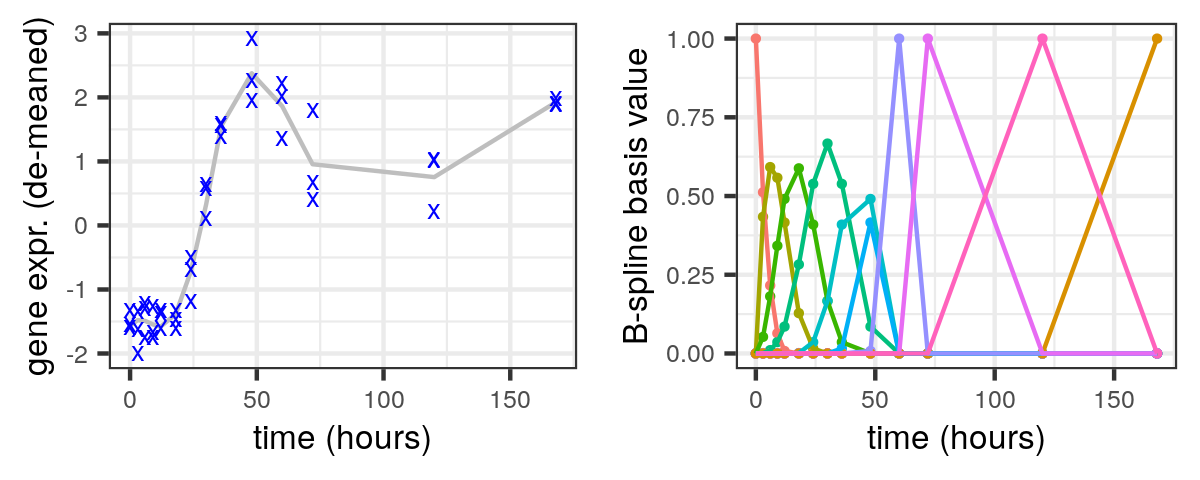
\includegraphics[width=0.980\linewidth,height=0.392\linewidth]{figure/example_genes-1} 

}

\caption[(Left) An example gene and its expression measured at 14 unique time points
    with three biological replicates at each time point.
     (Right) The cubic B-spline basis with 7 degrees of freedom,
    along with three indicator functions for the last three time points,
    $\timeindx = 72, 120, 168$]{(Left) An example gene and its expression measured at 14 unique time points
    with three biological replicates at each time point.
     (Right) The cubic B-spline basis with 7 degrees of freedom,
    along with three indicator functions for the last three time points,
    $\timeindx = 72, 120, 168$.}\label{fig:example_genes}
\end{figure}


\end{knitrout}
%

\todo{Connect the alpha range to the formula for expected number of clusters.
Also define the range of $\alpha$ here.  It would be good to make the
each section follow the same structure as much as possible.}

In this application, we expect {\em a priori} to uncover more distinct clusters
than in the iris data of the previous section. so we set $\alpha_0 = 6$ in the
initial GEM prior.

% $\gcoclustering(\eta)$, whose , given by
% \begin{align*}
% \gcoclustering{ij}(\eta)
% &= \expect{\q(\z\vert\eta)}{\ind{\z_{i} = \z_{j}}} \\
% &= \sum_{k=1}^{\kmax}\left(\expect{\q(\z_i\vert\eta)}{\z_{ik}}
% \expect{\q(\z_j\vert\eta)}{\z_{jk}}\right).
% \end{align*}

\todo{Define the co-clustering matrix before displaying it}

\subsection*{Quantity of interest: The co-clustering matrix}

For this model, we are particularly interested in which genes cluster together,
a quantity which we express through the following posterior co-clustering
matrix.  Let $\gcoclustering(\eta)\in\mathbb{R}^{\N\times\N}$ denote the matrix
whose $(i,j)$-th entry is the posterior probability that gene $i$ belongs to the
same cluster as gene $j$, given by \todo{This isn't right for $i=j$, is it?}
%
\begin{align*}
%
[\gcoclustering(\eta)]_{ij} =
\expect{\q(\z\vert\eta)}{\ind{\z_{i} = \z_{j}}}  =
\sum_{k=1}^{\kmax}\left(\expect{\q(\z_i\vert\eta)}{\z_{ik}}
\expect{\q(\z_j\vert\eta)}{\z_{jk}}\right).
%
\end{align*}
%
\figref{gene_initial_coclustering} displays the inferred co-clustering matrix
at $\alpha_0$.


Below, we evaluate the sensitivity of the inferred co-clustering matrix to
both parametric and functional perturbations to the stick distribution.

\newcommand{\MiceSmoothers}{
% moving this to appendix

\begin{knitrout}
\definecolor{shadecolor}{rgb}{0.969, 0.969, 0.969}\color{fgcolor}\begin{figure}[!h]

{\centering 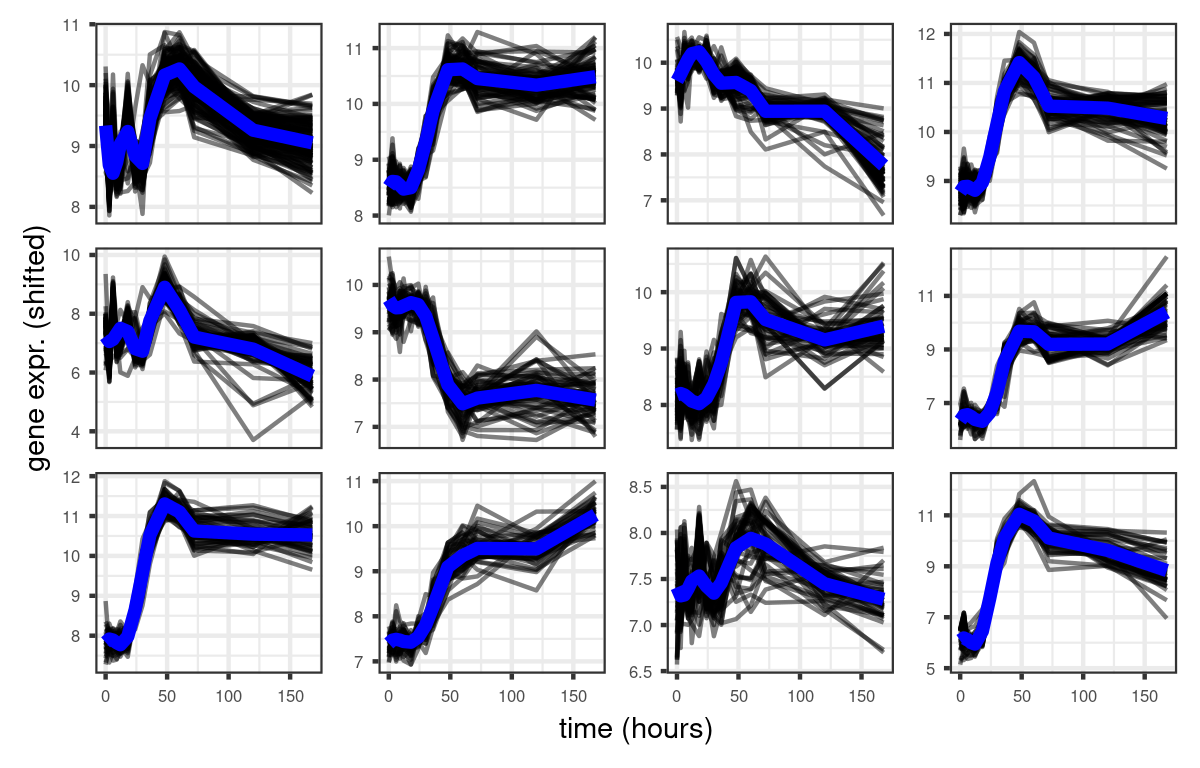
\includegraphics[width=0.980\linewidth,height=0.627\linewidth]{figure/gene_centroids-1} 

}

\caption[Inferred clusters in the mice gene expression dataset.
    Shown are the twelve most occupied clusters.
    In blue, the inferred cluster centroid.
    In grey, gene expressions averaged over replicates and
    shifted by their inferred intercepts]{Inferred clusters in the mice gene expression dataset.
    Shown are the twelve most occupied clusters.
    In blue, the inferred cluster centroid.
    In grey, gene expressions averaged over replicates and
    shifted by their inferred intercepts. }\label{fig:gene_centroids}
\end{figure}


\end{knitrout}
}



\begin{knitrout}
\definecolor{shadecolor}{rgb}{0.969, 0.969, 0.969}\color{fgcolor}\begin{figure}[!h]

{\centering 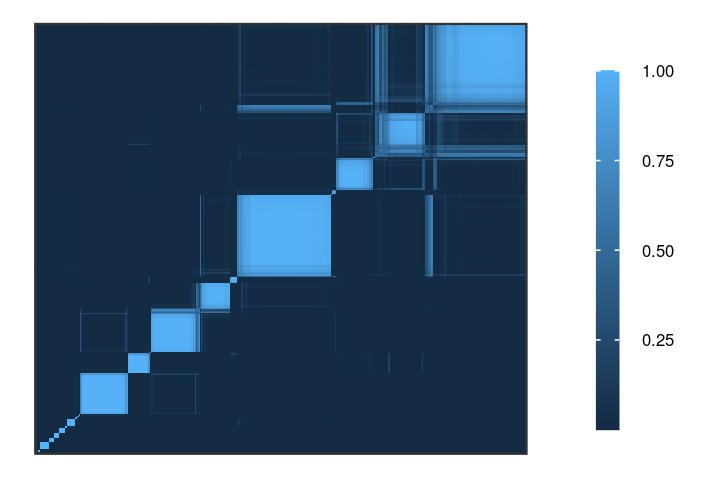
\includegraphics[width=0.588\linewidth,height=0.470\linewidth]{figure/gene_initial_coclustering-1} 

}

\caption[The inferred co-clustering matrix of gene expressions at $\alpha_0 = 6.$ ]{The inferred co-clustering matrix of gene expressions at $\alpha_0 = 6.$ }\label{fig:gene_initial_coclustering}
\end{figure}


\end{knitrout}


\subsubsection*{Sensitivity of co-clustering to $\alpha$}

We first evaluate the sensitivity of the co-clustering matrix $\gcoclustering$
to the choice of $\alpha$ in the GEM prior. We formed the linear approximation
at $\alpha_0 = 6$ and computed the change in co-clustering under the linearized
variational parameters $\etalinglobal(\alpha)$, at $\alpha =
0.1$ and $\alpha = 12$. At $\alpha =
0.1$ the prior is concentrated, with only two clusters expected
under the GEM prior; at $\alpha = 12$, more than fifty are
expected.

\todo{Say that therefore $\gclustersabbr$ is non-robust, but we don't really
care about it here.}


% Let $\gcoclustering^0 := \gcoclustering(\etaopt(\alpha_0))$ be the co-clustering matrix inferred at $\alpha_0$,
% and let $\Delta\gcoclustering(\eta) :=
% \gcoclustering(\eta) - \gcoclustering^0$.

%(Note that the co-clustering matrix as a posterior quantity depends on only expectations of $\z$.
% We write $\gcoclustering(\etalinglobal)$ with the
% understanding that the coclustering matrix is a function of global parameters $\etaglob$ only through its corresponding local parameters $\eta_\z$).

\todo{Briefly explain how it can be that the co-clustering can be
robust even though the number of clusters is not.}

Despite this wide prior range, for either $\alpha$, the change in the posterior
co-clustering matrix is minuscule (\figref{gene_alpha_coclustering}): the
largest absolute changes in the co-clustering matrix is of order $10^{-2}$.
Refitting the approximate posterior at $\alpha = 0.1$ and
$\alpha = 12$ confirms the insensitivity predicted by the
linearized variational global parameters. Beyond capturing insensitivity, the
linearized parameters were also able to approximate the sign and size of the
changes in the individual entries of the coclustering matrix (these changes
albeit small).


\begin{knitrout}
\definecolor{shadecolor}{rgb}{0.969, 0.969, 0.969}\color{fgcolor}\begin{figure}[!h]

{\centering 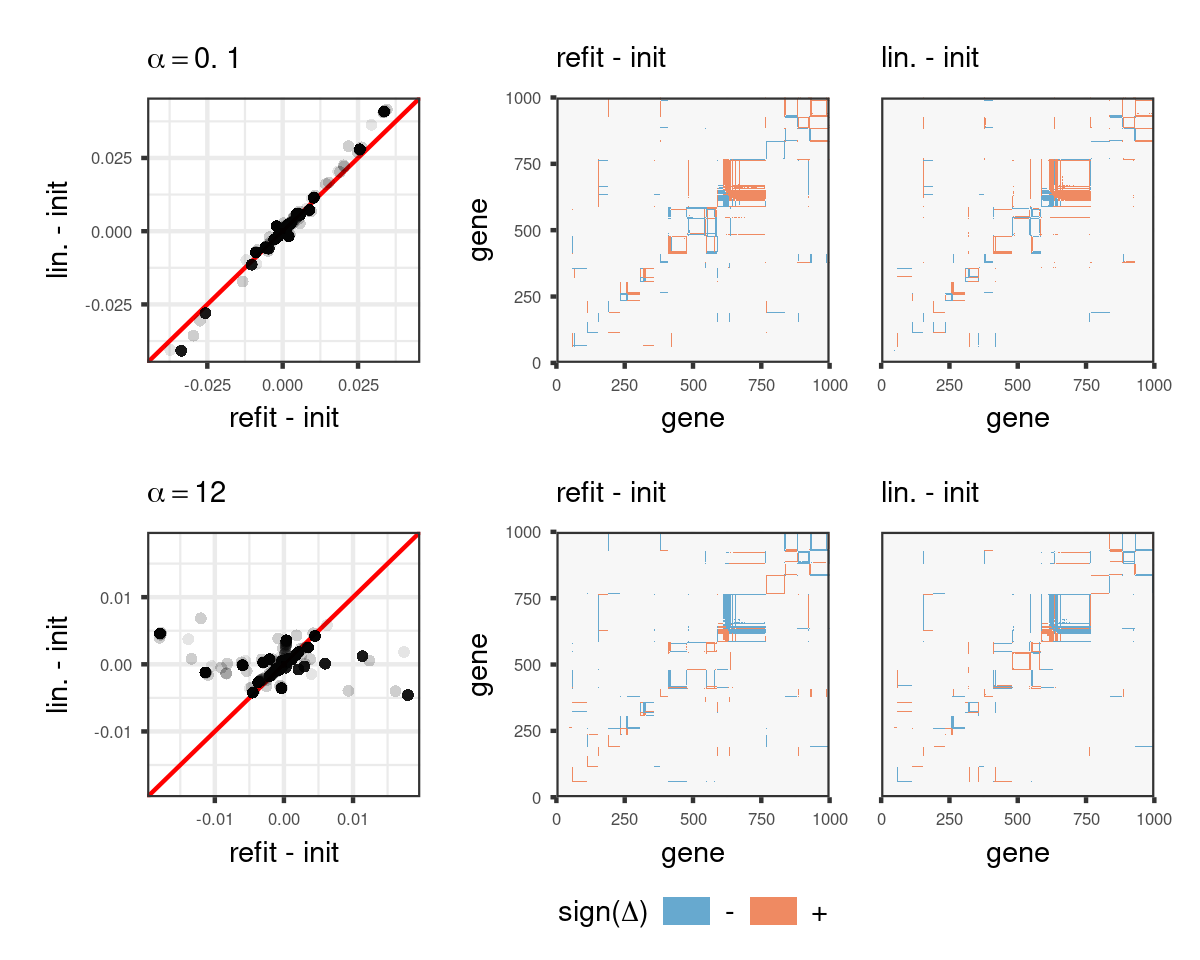
\includegraphics[width=0.980\linewidth,height=0.784\linewidth]{figure/gene_alpha_coclustering-1} 

}

\caption[Differences in the
     co-clustering matrix at $\alpha = 0.1$ (top row)
     and $\alpha = 12$ (bottom row),
     relative to the co-clustering matrix at $\alpha_0 = 6$.
     (Left) a scatter plot of differences under the linear approximation
     against differences after refitting, where
     each point represents an entry of the co-coclustering matrix.
     Note the scales of the axes:
     the largest change in an entry of the co-clustering matrix is
     $\approx 0.03$.
     (Middle) sign changes in the co-clustering matrix observed after refitting.
     (Right) the changes under the linearly approximated variational
     parameters.
     For visualization, changes with absolute value $< 1e-5$ are not colored]{Differences in the
     co-clustering matrix at $\alpha = 0.1$ (top row)
     and $\alpha = 12$ (bottom row),
     relative to the co-clustering matrix at $\alpha_0 = 6$.
     (Left) a scatter plot of differences under the linear approximation
     against differences after refitting, where
     each point represents an entry of the co-coclustering matrix.
     Note the scales of the axes:
     the largest change in an entry of the co-clustering matrix is
     $\approx 0.03$.
     (Middle) sign changes in the co-clustering matrix observed after refitting.
     (Right) the changes under the linearly approximated variational
     parameters.
     For visualization, changes with absolute value $< 1e-5$ are not colored. }\label{fig:gene_alpha_coclustering}
\end{figure}


\end{knitrout}

\subsubsection*{Sensitivity of co-clustering to a functional perturbation}


\begin{knitrout}
\definecolor{shadecolor}{rgb}{0.969, 0.969, 0.969}\color{fgcolor}\begin{figure}[!h]

{\centering 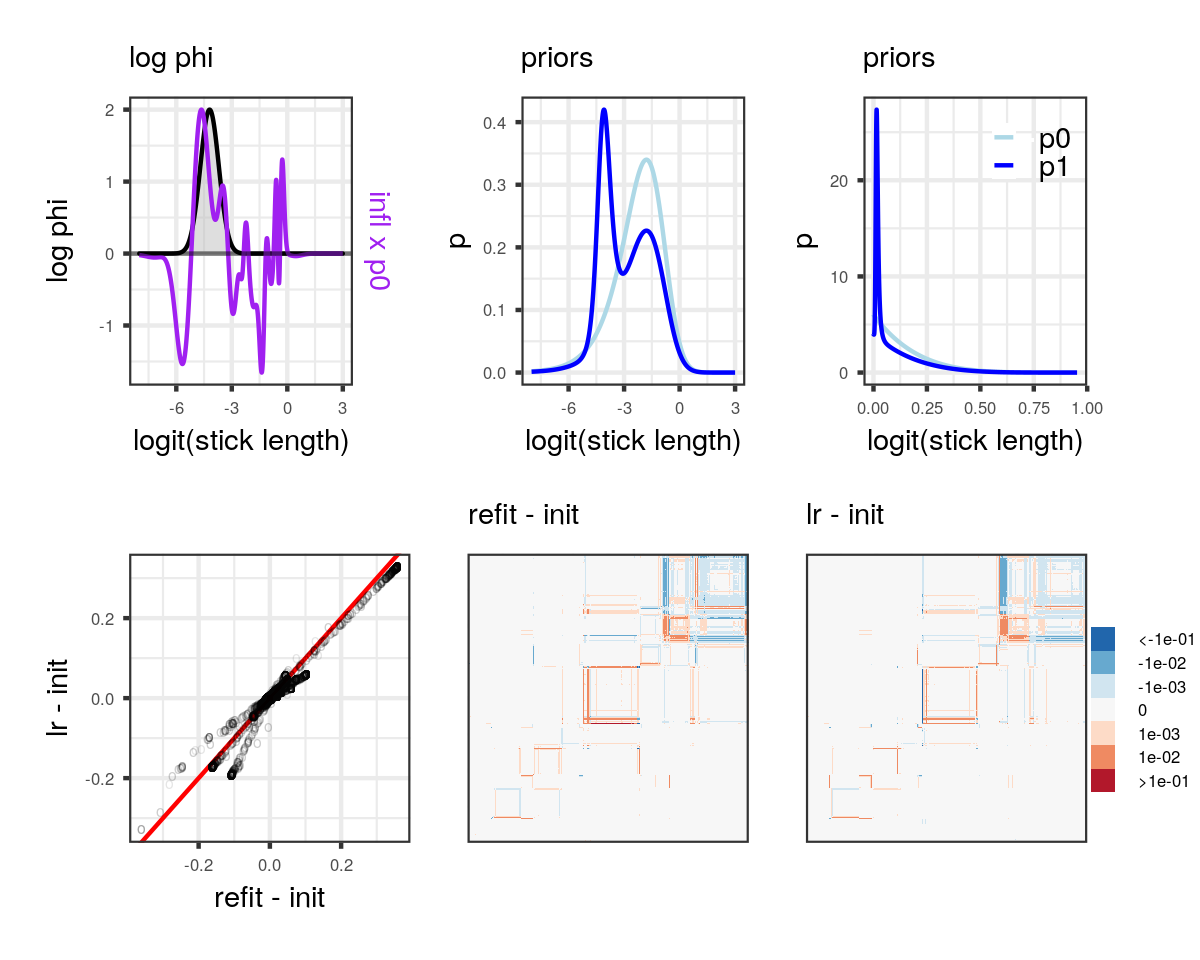
\includegraphics[width=0.980\linewidth,height=0.823\linewidth]{figure/gene_fpert_coclustering-1} 

}

\caption[Effect on the co-clustering matrix after a multiplicative functional
     perturbation.
     (Top left) the perturbation $\phi$ in grey,
     and the influence function in purple.
     (Top right) the effect of this perturbation on the prior density.
     (Bottom) the effect of this perturbation on
    the coclustering matrix.
    Note the scale of the scatterplot axes compared with
    the scatterplots in \figref{gene_alpha_coclustering}]{Effect on the co-clustering matrix after a multiplicative functional
     perturbation.
     (Top left) the perturbation $\phi$ in grey,
     and the influence function in purple.
     (Top right) the effect of this perturbation on the prior density.
     (Bottom) the effect of this perturbation on
    the coclustering matrix.
    Note the scale of the scatterplot axes compared with
    the scatterplots in \figref{gene_alpha_coclustering}. }\label{fig:gene_fpert_coclustering}
\end{figure}


\end{knitrout}


\begin{knitrout}
\definecolor{shadecolor}{rgb}{0.969, 0.969, 0.969}\color{fgcolor}\begin{figure}[!h]

{\centering 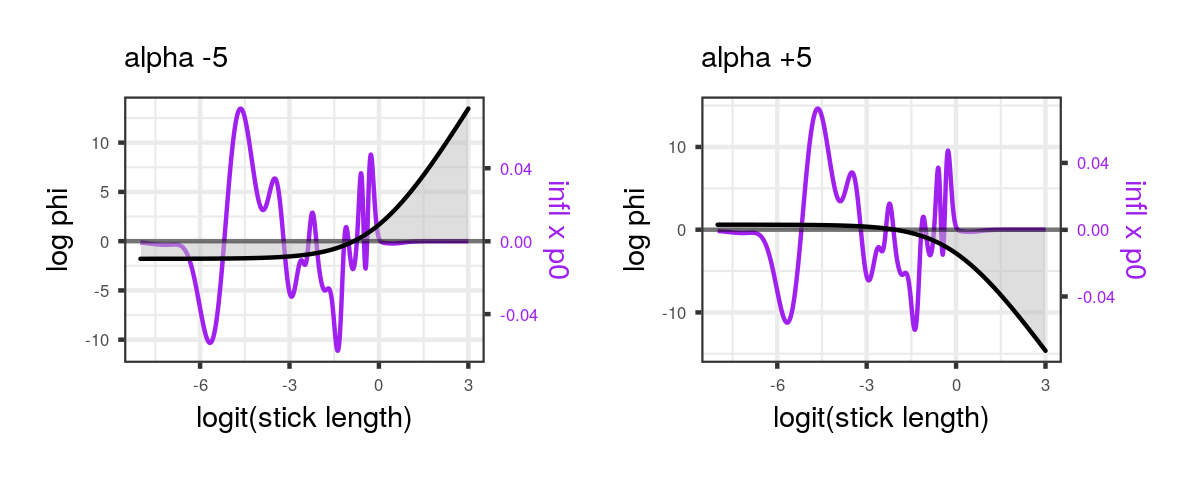
\includegraphics[width=0.882\linewidth,height=0.423\linewidth]{figure/alpha_pert_logphi-1} 

}

\caption[The multiplicative perturbations $\phi_\alpha(\cdot)$ that
    corresponds to decreasing (left) or increasing (right)
    the $\alpha$ parameter]{The multiplicative perturbations $\phi_\alpha(\cdot)$ that
    corresponds to decreasing (left) or increasing (right)
    the $\alpha$ parameter. }\label{fig:alpha_pert_logphi}
\end{figure}


\end{knitrout}

As in \secref{results_iris}, we now investigate whether the co-clustering matix
is robust to deviations from the Beta prior. To use \corref{etafun_worst_case} as
well as to produce an easily-visualized influence function, we must choose a
univariate summary of the $\ngenes^2$-dimensional co-clustering matrix. We use
the sum of the eigenvalues of the symmetrically normalized graph Laplacian, as
given by
%
\begin{align*} \laplacianevsum(\eta) = \text{Tr}\left( I - D(\eta)^{-1/2}
\gcoclustering(\eta) D(\eta)^{-1/2} \right), \end{align*}
%
where $D(\eta)^{-1/2}$ is the diagonal matrix with entries $d_i =
\sum_{j=1}^{\ngenes}[\gcoclustering(\eta)]_{ij}$. The quantity $\laplacianevsum$
is differentiable, and has close connection with the number of distinct
components in a graph~\citep{luxburg:2007:spectralcluster}. We expect that prior
changes that produce large changes in $\laplacianevsum$ will also produce large
changes in the full co-clustering matrix.

% Is this important?
%(And recall that the trace of a matrix is equivalent to the sum of its eigenvalues).

In \figref{gene_fpert_coclustering}, we use the influence function for
$\laplacianevsum$ to construct a nonparametric prior perturbation which we
expect to have a large, positive effect.  The resulting prior does indeed
produce changes an order of magnitude larger than those produced by $\alpha$
perturbations shown in \figref{gene_alpha_coclustering}, and the approximation
is able to capture the qualitative changes.  The influence function is able to
capture why $\alpha$ perturbations were unable to produce large changes in this
case: \figref{alpha_pert_logphi} shows that changing $\alpha$ (as in
\exref{beta_inf_norm}) induces large changes in the prior only where the
influence function is small.


However, even with the selected functional perturbation,
the size of the differences in the co-clustering matrix remains modest.
It is unlikely that any conclusions derived from the co-clustering matrix would have changed after the functional perturbation.
The co-clustering matrix appears insensitive to perturbations in the stick-breaking distribution.

Finally, the computational cost of linearizing the variational parameters is favorable compared with refitting (\tabref{mice_timing}).
Forming the linear approximation, which requires a Hessian inversion,
took 3-4 seconds; subsequent evaluations of $\etalinglobal$ take milliseconds. Conversely, refitting the model after a prior perturbation can take more than 30 seconds.

\begin{table}[tb]
\centering
\caption{Compute time of results on the mice data set. }
\tablabel{mice_timing}
\begin{tabular}{|r|r|}
    \hline
    & time (seconds) \\
    \hline
    Initial fit & 27 \\
    \hline
    Hessian solve for $\alpha$ sensitivity &
        3.2\\
    Linear approx. $\etalinglobal(\alpha)$ for $\alpha = 0.1$ &
        0.00098\\
    Linear approx. $\etalinglobal(\alpha)$ for $\alpha = 12$ &
        0.0011\\
    Refit $\etaopt(\alpha)$ for $\alpha = 0.1$ &
        46\\
    Refit $\etaopt(\alpha)$ for $\alpha = 12$ &
        12\\
    \hline
    The influence function & 3.4\\
    Hessian solve for $\phi$ perturbation &
        2.8\\
    Linear approx. $\etalin(\t)$ at $\t = 1$ &
        0.00095\\
    Refit $\etaopt(\t)$ at $\t = 1$ &
        24\\
    \hline
\end{tabular}
\end{table}
